%%%%%%%%%%%%%%%%%%%%%%%%%%%%%%%%%%%%%%%%%%%%%%%%%%%%%%%%%%%%%%%%%%%%%
\section{Motivating Example and Background} \label{sect:background}
%%%%%%%%%%%%%%%%%%%%%%%%%%%%%%%%%%%%%%%%%%%%%%%%%%%%%%%%%%%%%%%%%%%%%

This section motivates our work by means of example and reviews the background concepts that form the basis for our discussion in this paper.

%%%%%%%%%%%%%%%%%%%%%%%%%%%%%%%%%%%%%%%%%%%%%%
\subsection{Motivating Example} 
\label{sect:bg-courseman-eg}
%%%%%%%%%%%%%%%%%%%%%%%%%%%%%%%%%%%%%%%%%%%%%%

% ducmle: OLD
%\begin{figure*}[ht]
%	\begin{center}
%		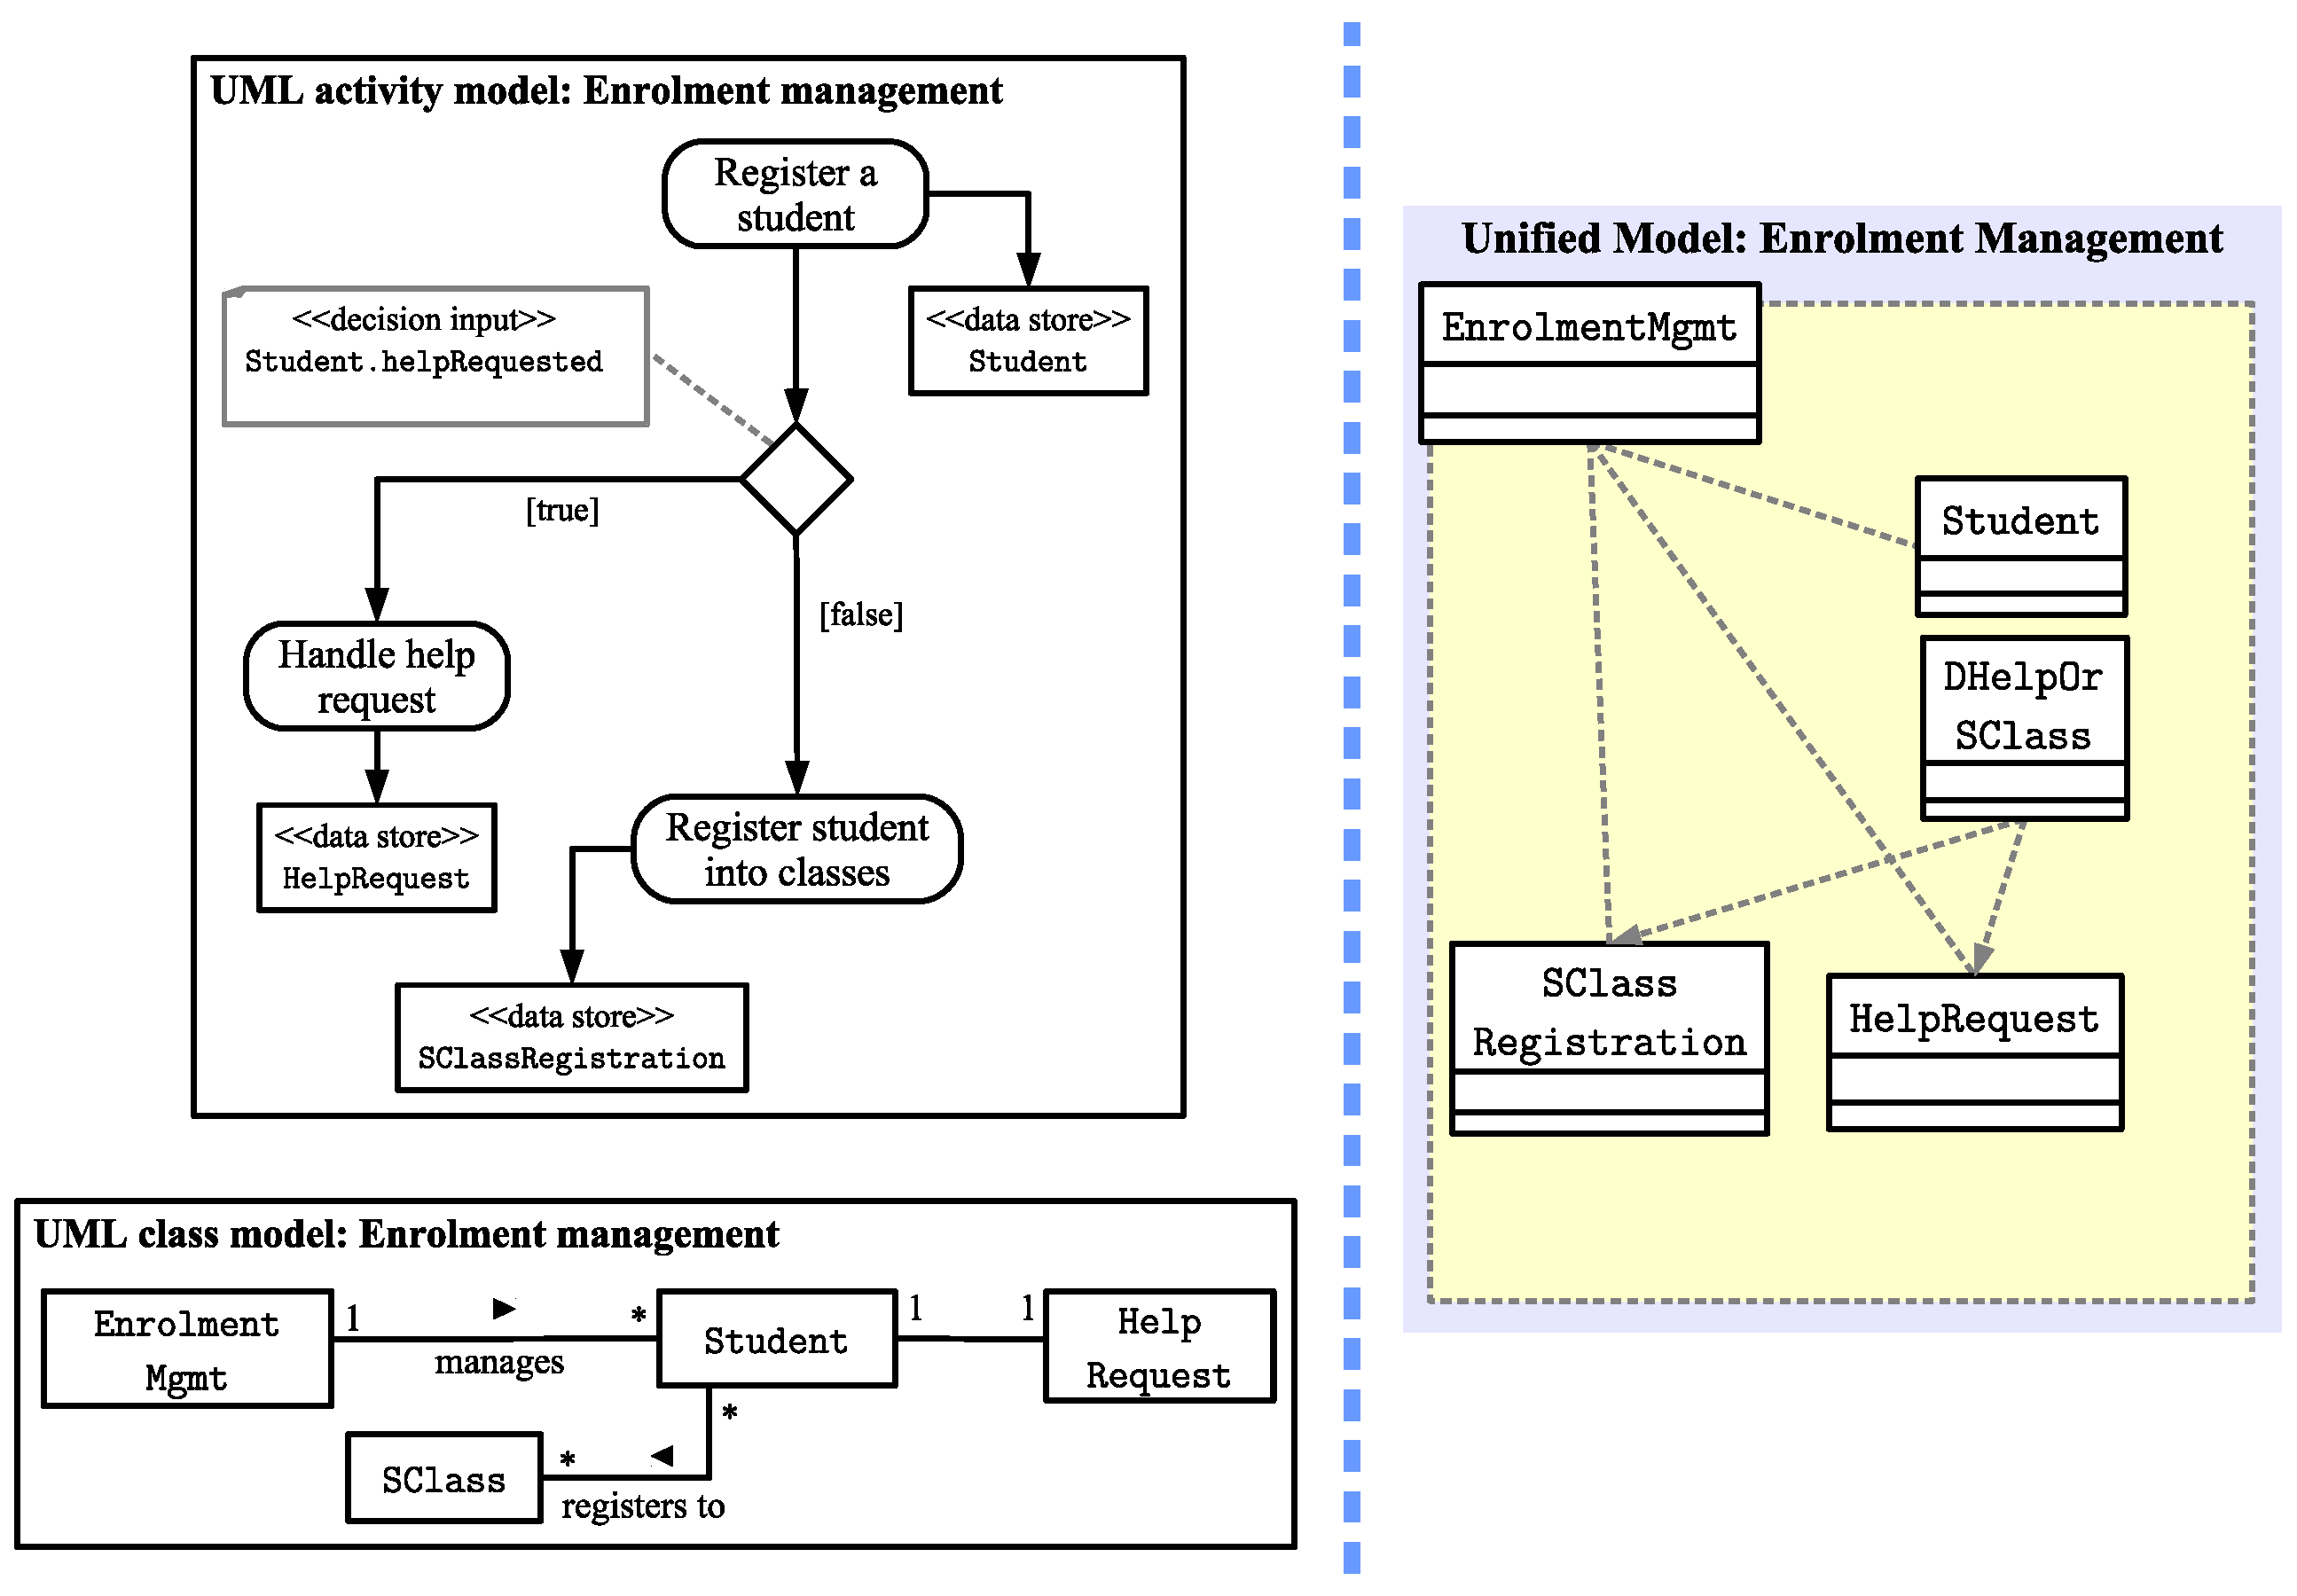
\includegraphics[scale=0.28]{motivatingExample}
%	\end{center}
%	\caption{Simplified UML/OCL class and activity diagrams to specify a \courseman software variant that handles the enrolment management activity.} %
%	\label{fig:motivatingExample}
%\end{figure*} 
We adapt a compact and essential software domain from a previous work \cite{le_domain_2018}, named course management domain (\courseman) as our motivating example. We will introduce here the basic \courseman requirements and use it to illustrate the background concepts. In the rest of the paper, we will use this example and, where necessary, some extensions of it to illustrate our proposed method.

\begin{figure}[th]
\begin{center}
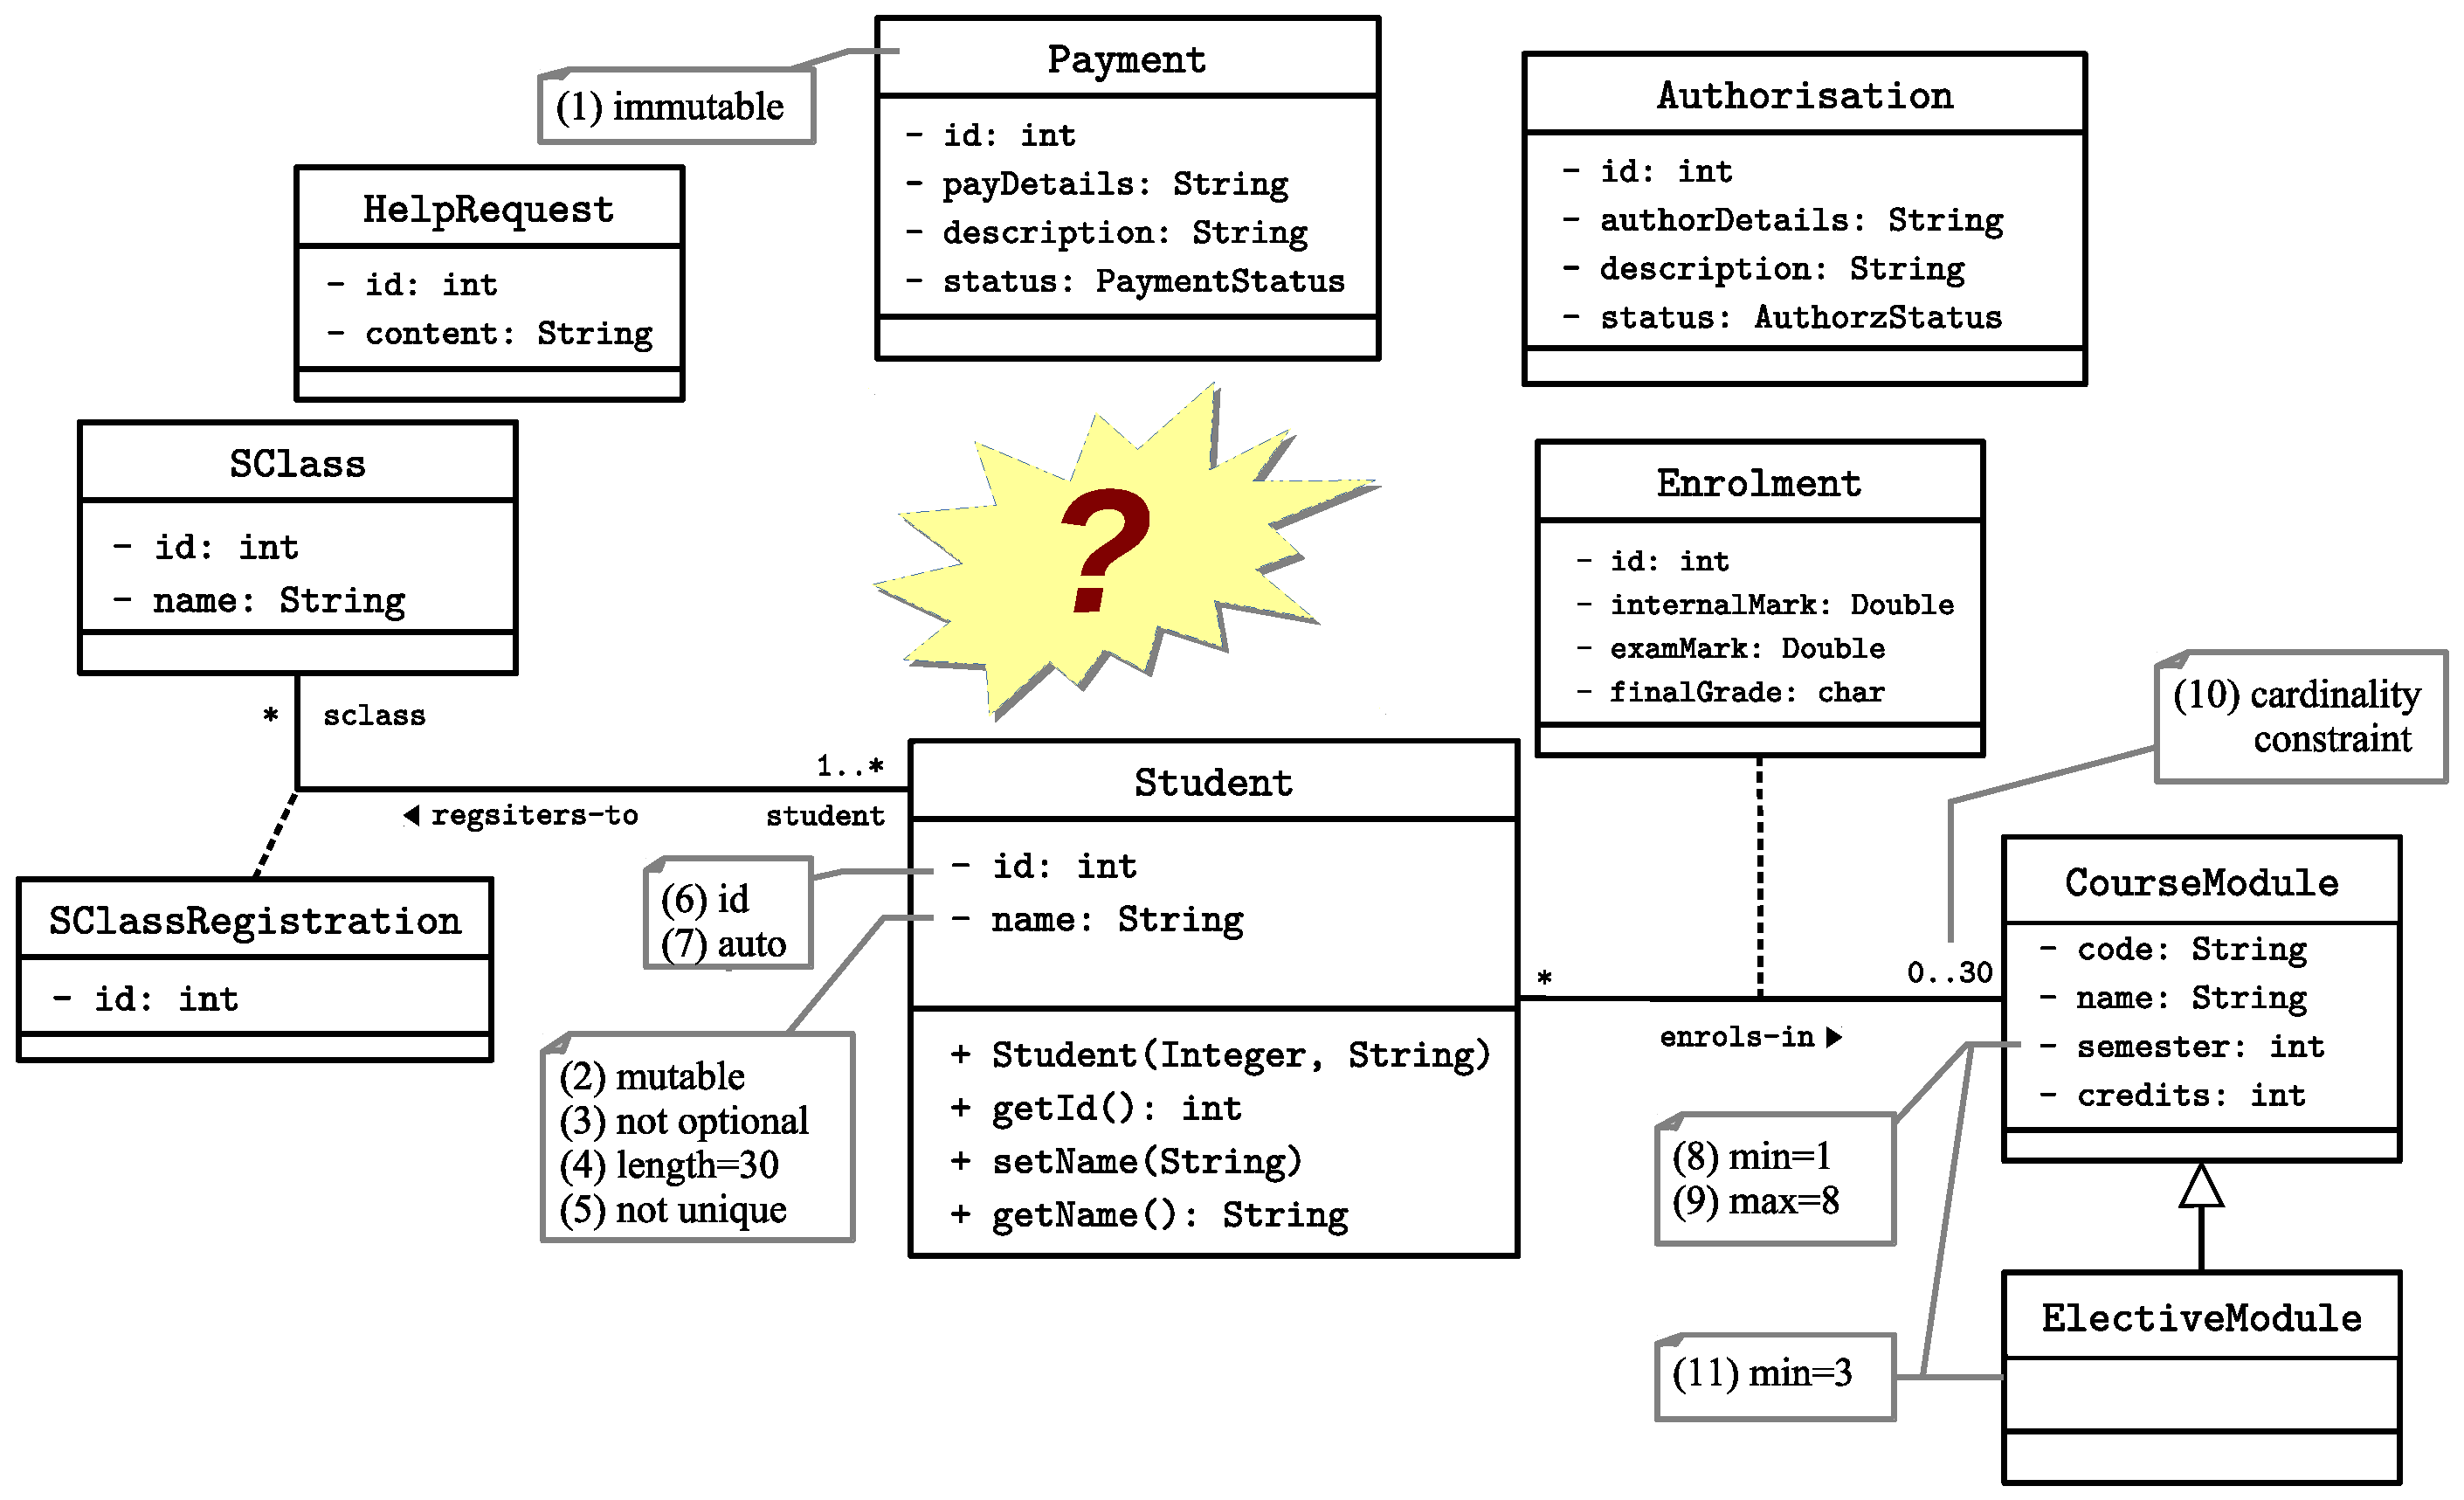
\includegraphics[scale=0.28]{motivating-example}
\end{center}
\caption{The essential domain model of \courseman.}
\label{fig:motivatingExample}
\end{figure}

The bottom part of Figure~\ref{fig:motivatingExample} shows four classes and two association classes of \Name{CourseMan}. Class \clazz{Student} represents students that register to study in an academic institution. Class \clazz{CourseModule} represents the course modules that are offered by the institution. Class \clazz{ElectiveModule} represents a specialised type of \clazz{CourseModule}. Class \clazz{SClass} represents the student class type for students to choose. Association class \clazz{\clazz{SClass}Registration} captures details about the many-many association between \clazz{Student} and \clazz{SClass}. Finally, association class \clazz{Enrolment} captures details about the many-many association between \clazz{Student} and \clazz{CourseModule}.
The top part of Figure~\ref{fig:motivatingExample} (the area containing a star-like shape labelled ``?'') shows three other classes that are intended to capture the design of an enrolment management activity. Suppose that we know some design details (the attributes shown in the figure) and the following description about these classes:
%
\begin{itemize}[noitemsep]
  \item \clazz{HelpRequest}: captures data about help information provided to students.
  \item \clazz{Payment}: captures data about payment for the intuition fee that a student needs to make.
  \item \clazz{Authorisation}: captures data about the decision made by an enrolment officer concerning whether or not to allow a student to undertake the registered course modules.
  % paragraph break
  %\\
\end{itemize}

We illustrate below how a number of common invariant constraints on \clazz{Student} and \clazz{CourseModule} are expressed in OCL \cite{omg_object_2014}. Other constraints are expressed using more complex OCL expressions and techniques, whose details (see \cite{le_domain_2018}) are beyond the scope of this paper.

%
\begin{lstrulex}
context (@\hterm{Student inv}@):
  -- constraint (@\hterm{(3)}@):
  not(name.oclIsUndefined()) and 
  -- constraint (@\hterm{(4)}@):
  name.size() <= 30

context (@\hterm{CourseModule inv}@):
  -- constraint (@\hterm{(8)}@):
  semester >= 1 and 
  -- constraint (@\hterm{(9)}@):
  semester <= 8
\end{lstrulex}

\begin{figure}[th]
	\begin{center}
		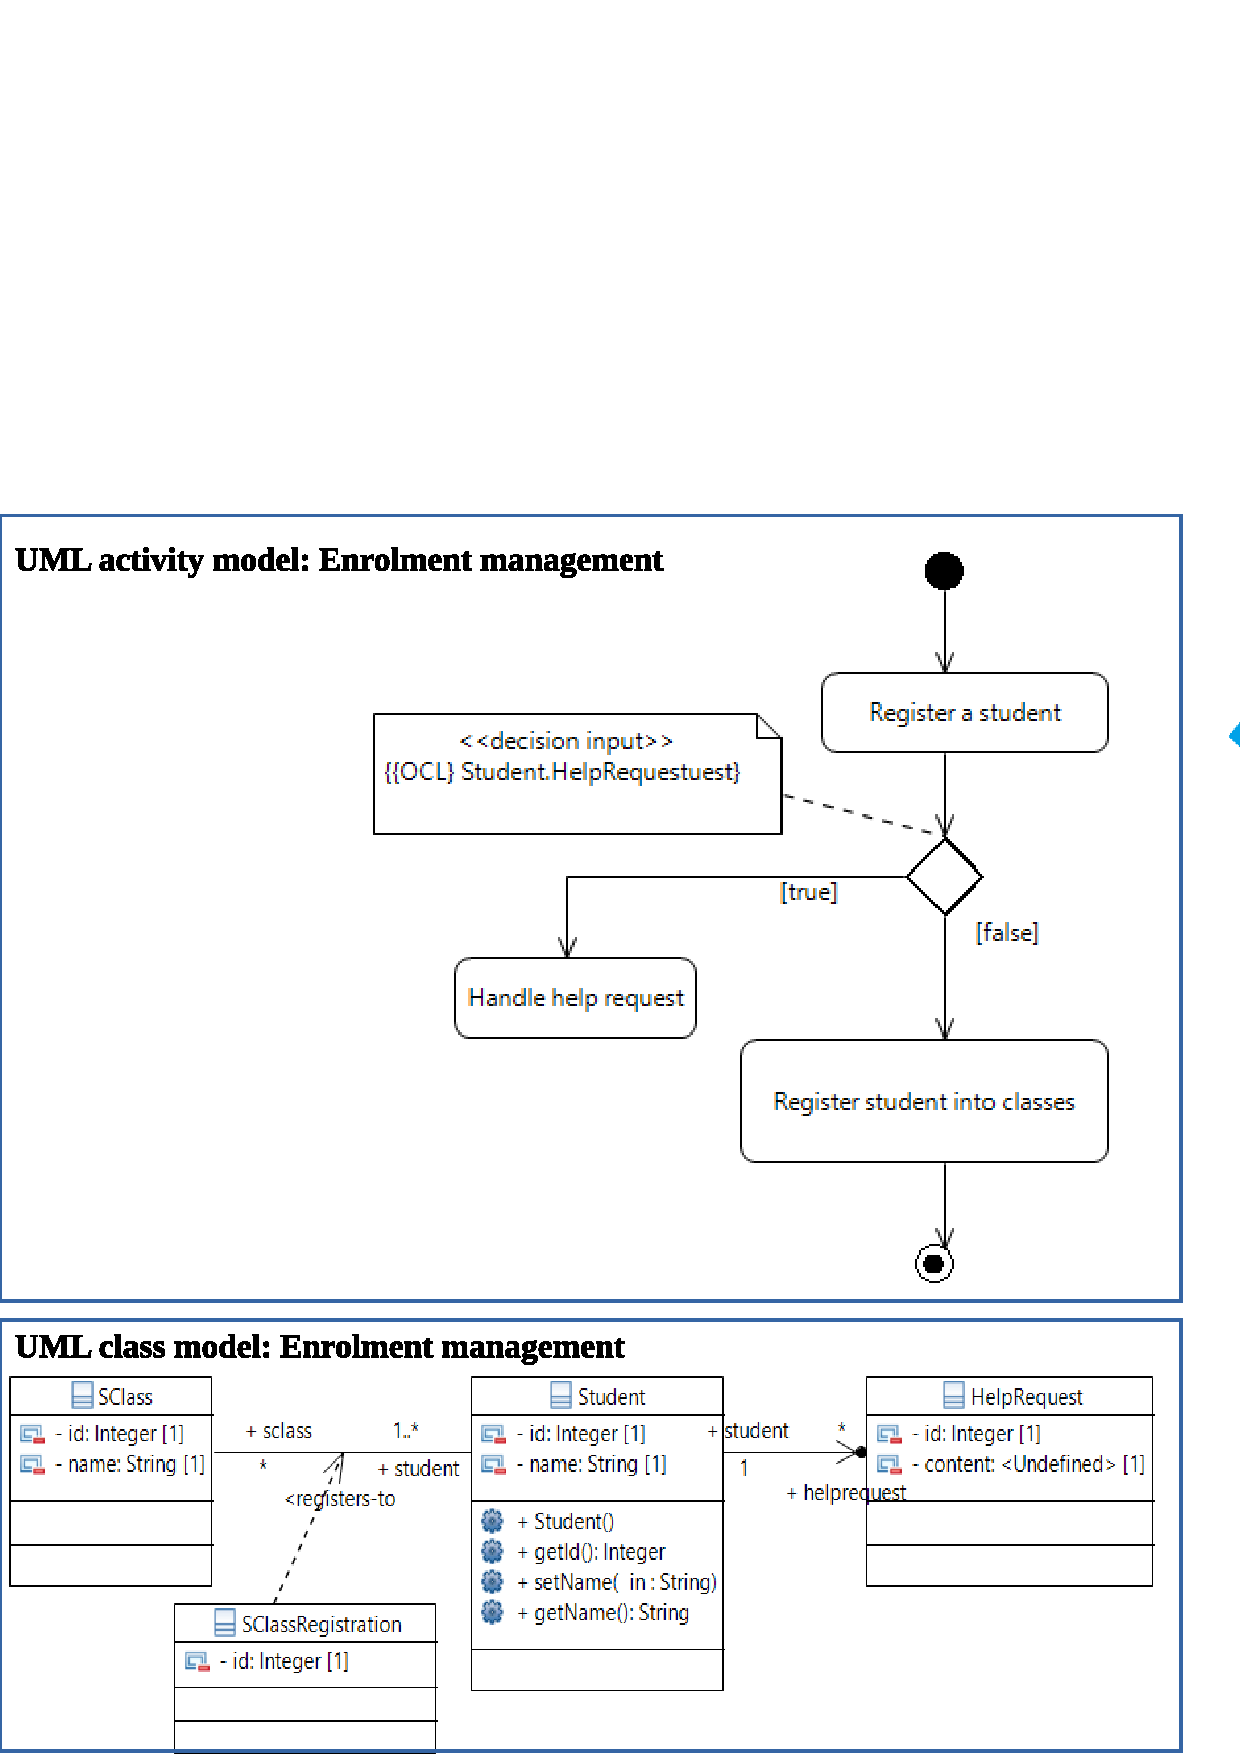
\includegraphics[scale=0.35]{motivating-example2}
	\end{center}
	\caption{Combining structural and behavioural \courseman models.}
	\label{fig:motivatingExample2}
\end{figure}

In practical applications, the class model is often combined with a behavioral model (\eg a UML activity diagram) to describe a unified view of the domain requirements. Throughout this paper, we will refer to this combined model as \textit{unified domain model}. For instance, the left-hand side of Fig.~\ref{fig:motivatingExample2} illustrates the combination of a simplied class diagram of \courseman (displayed at the bottom) and an activity diagram of the enrolment management function. This activity involves registering \clazz{Student}s, enrolling them into \clazz{CourseModule}s and registering them into \clazz{SClass}es. In addition, it would allow a \clazz{Student} to raise a \clazz{HelpRequest} during the enrolment process. 
The right-hand side of Fig.~\ref{fig:motivatingExample2} depicts an unspecified unified domain model of the \courseman example. What this model entails and how this can be specified are the main questions that we seek to answer in this paper. We will state shortly a number of research questions relating to this model that we will specifically focus on investigating.

%Class \clazz{Student} represents the domain concept Student%
%\footnote{use \clazz{fixed~font} for model elements and normal font for concepts.}. %
%Class \clazz{Course} represents the Courses%
%\footnote{use class/concept name as countable noun to identify instances.} %
%that are offered to students. Class \clazz{SClass} represents types of classes (\eg morning, afternoon, and evening) that \clazz{Student}s
%can choose. 

%Class \clazz{EnrolmentMgmt} represents the enrolment management activity. This essentially involves registering \clazz{Student}s, enrolling them into \clazz{CourseModule}s and registering them into \clazz{SClass}es. In addition, it allows each \clazz{Student} to raise a \clazz{HelpRequest}. Throughout this paper, we will discuss different variants of this activity.
%The right-hand side of Fig.~\ref{fig:motivatingExample} depicts an activity diagram that captures behavioral aspects from the enrolment management activity.

% + (done) TODO: Duc
% - copy example from the 2018 Journal paper here
% - add the activity diagram EnrolmentMgmt (in this paper, we will extend this basic example to handle all the basic activity diagram patterns)

%%%%%%%%%%%%%%%%%%%%%%%%%%%%%%%%%%%%%%%%%%%%%%
\subsection{Domain Models in the Annotation-Based Domain Specific Language \dcsl}
\label{sect:bg-dcsl}
%%%%%%%%%%%%%%%%%%%%%%%%%%%%%%%%%%%%%%%%%%%%%%

\abbrv{Annotation-Based Domain Specific Language}{\textbf{aDSL}} is coined in~\cite{nosal_language_2016} as an attempt to formalise the notion of fragmentary, internal DSL~\cite{fowler_domain-specific_2010} for the use of annotation to define DSLs. An aDSL is defined based on an OOPL's abstract syntax model~\cite{le_domain_2018} that consists of the following meta-concepts: class, field, method, parameter, annotation, and property. These meta-concepts are common to two popular host OOPLs: Java~\cite{gosling_java_2014} and C\#~\cite{hejlsberg_c_2010}.

%
We stated in~\cite{le_domain_2018} that using aDSL for DDD brings three important benefits for domain modeling: feasibility, productivity, and understandability. Feasibility comes from the fact the domain model is feasible for implementation in a host OOPL. Productivity is achieved by leveraging the host language platform tools and libraries to process and transform the domain model into other forms suitable for constructing the software. Understandability of the domain model code is enhanced with the introduction of domain-specific annotations.

Within the scope of this paper and based on the DSL classification in~\cite{kleppe_software_2008}, we differentiate between two types of aDSL: horizontal and vertical aDSLs.
A \textit{vertical aDSL} targets a bounded real-world (vertical) domain. In contrast, a \textit{horizontal aDSL} (\aka technical aDSL) targets a technical (low-level) domain, whose concepts describe the patterns that often underlie a class of vertical domains that share common features. 
%Thus, horizontal DSL has a wide scope of application because it is used to build a class of vertical DSLs.
More specifically, a horizontal aDSL is a DSL internal to a host OOPL, whose domain is a technical one and that uses a set of annotations to model the domain concepts.

%For example, the \courseman's domain model presented in Figure~\ref{fig:arch-model-courseman} can be used as the meta-model for a vertical aDSL for the \courseman~domain. We discussed in~\cite{le_domain_2018} how this domain model is expressed in a horizontal aDSL named \dcsl. A partial \dcsl's domain model of \courseman~is shown in Figure~\ref{fig:dcsl_courseman}. We will review \dcsl~and explain this example in the next subsection.
% In Section~\ref{sect:agl}, we propose another horizontal aDSL for expressing activity graphs. 

\abbrv{Domain class specification language}{\name{DCSL}}~\cite{le_domain_2018} is a horizontal aDSL that we developed to express domain models.
A key feature of \name{DCSL} is that its meta-concepts model the generic domain terms that are composed of the core OOPL meta-concepts and constraints. More specifically, meta-concept \textbf{Domain Class} is composed of meta-concept \clazz{Class} and a constraint captured by an annotation named \clazz{DClass}. This constraint states whether or not the class is mutable. Similarly, meta-concept \textbf{Domain Field} is composed of meta-concept \clazz{Field} with a set of state space constraints. 
These constraints are represented by an annotation named \clazz{DAttr}. 
Meta-concept \textbf{Associative Field} represents Domain Field that realises one end of an association between two domain classes. \dcsl~supports all three types of association: one-to-one (\abbr one-one), one-to-many (\abbr one-many) and many-to-many (\abbr many-many). 
Finally, meta-concept \textbf{Domain Method} is composed of \clazz{Method} with a certain behavior type. The essential behavior types are represented by an annotation named \clazz{DOpt} and another annotation named \clazz{AttrRef}. The latter references the domain field that is the primary subject of a method's behavior.

Syntactically, we write a \dcsl~model directly using the host OOPL's syntax. For exposition purposes, however, we write this model using an extended UML graphical notation that uses a \textit{structured text box} for writing annotations. Specifically, nonannotation elements are drawn using the usual UML class diagram notation. On the other hand, the annotation elements are drawn using UML note box. Annotation assignment is represented by a dashed grey line, whose target element end is marked with the attachment symbol (\drawFilledRect[gray]{0.15cm}{0.15cm}). The note box content has the form $ A \; \{ props \} $, where $ A $ is the annotation name and $ props $ is a property listing. Each entry specifies the initialisation of a property to a value. If this value is another annotation element then this element is written using a nested, borderless note box. The entries are separated by either a next line or a comma (`,') character.

Another feature of the above notation is the use of a virtual (dashed) association line to represent a pair of \clazz{DAssoc} elements that help realise the association ends of an association. This association line is more compact and thus helps significantly ease drawing and improves readability of the model. 
We will often use the term ``association'' to refer this association line and the \Name{DCSL} model elements that realise it.

\begin{figure}[ht]
	\centering
	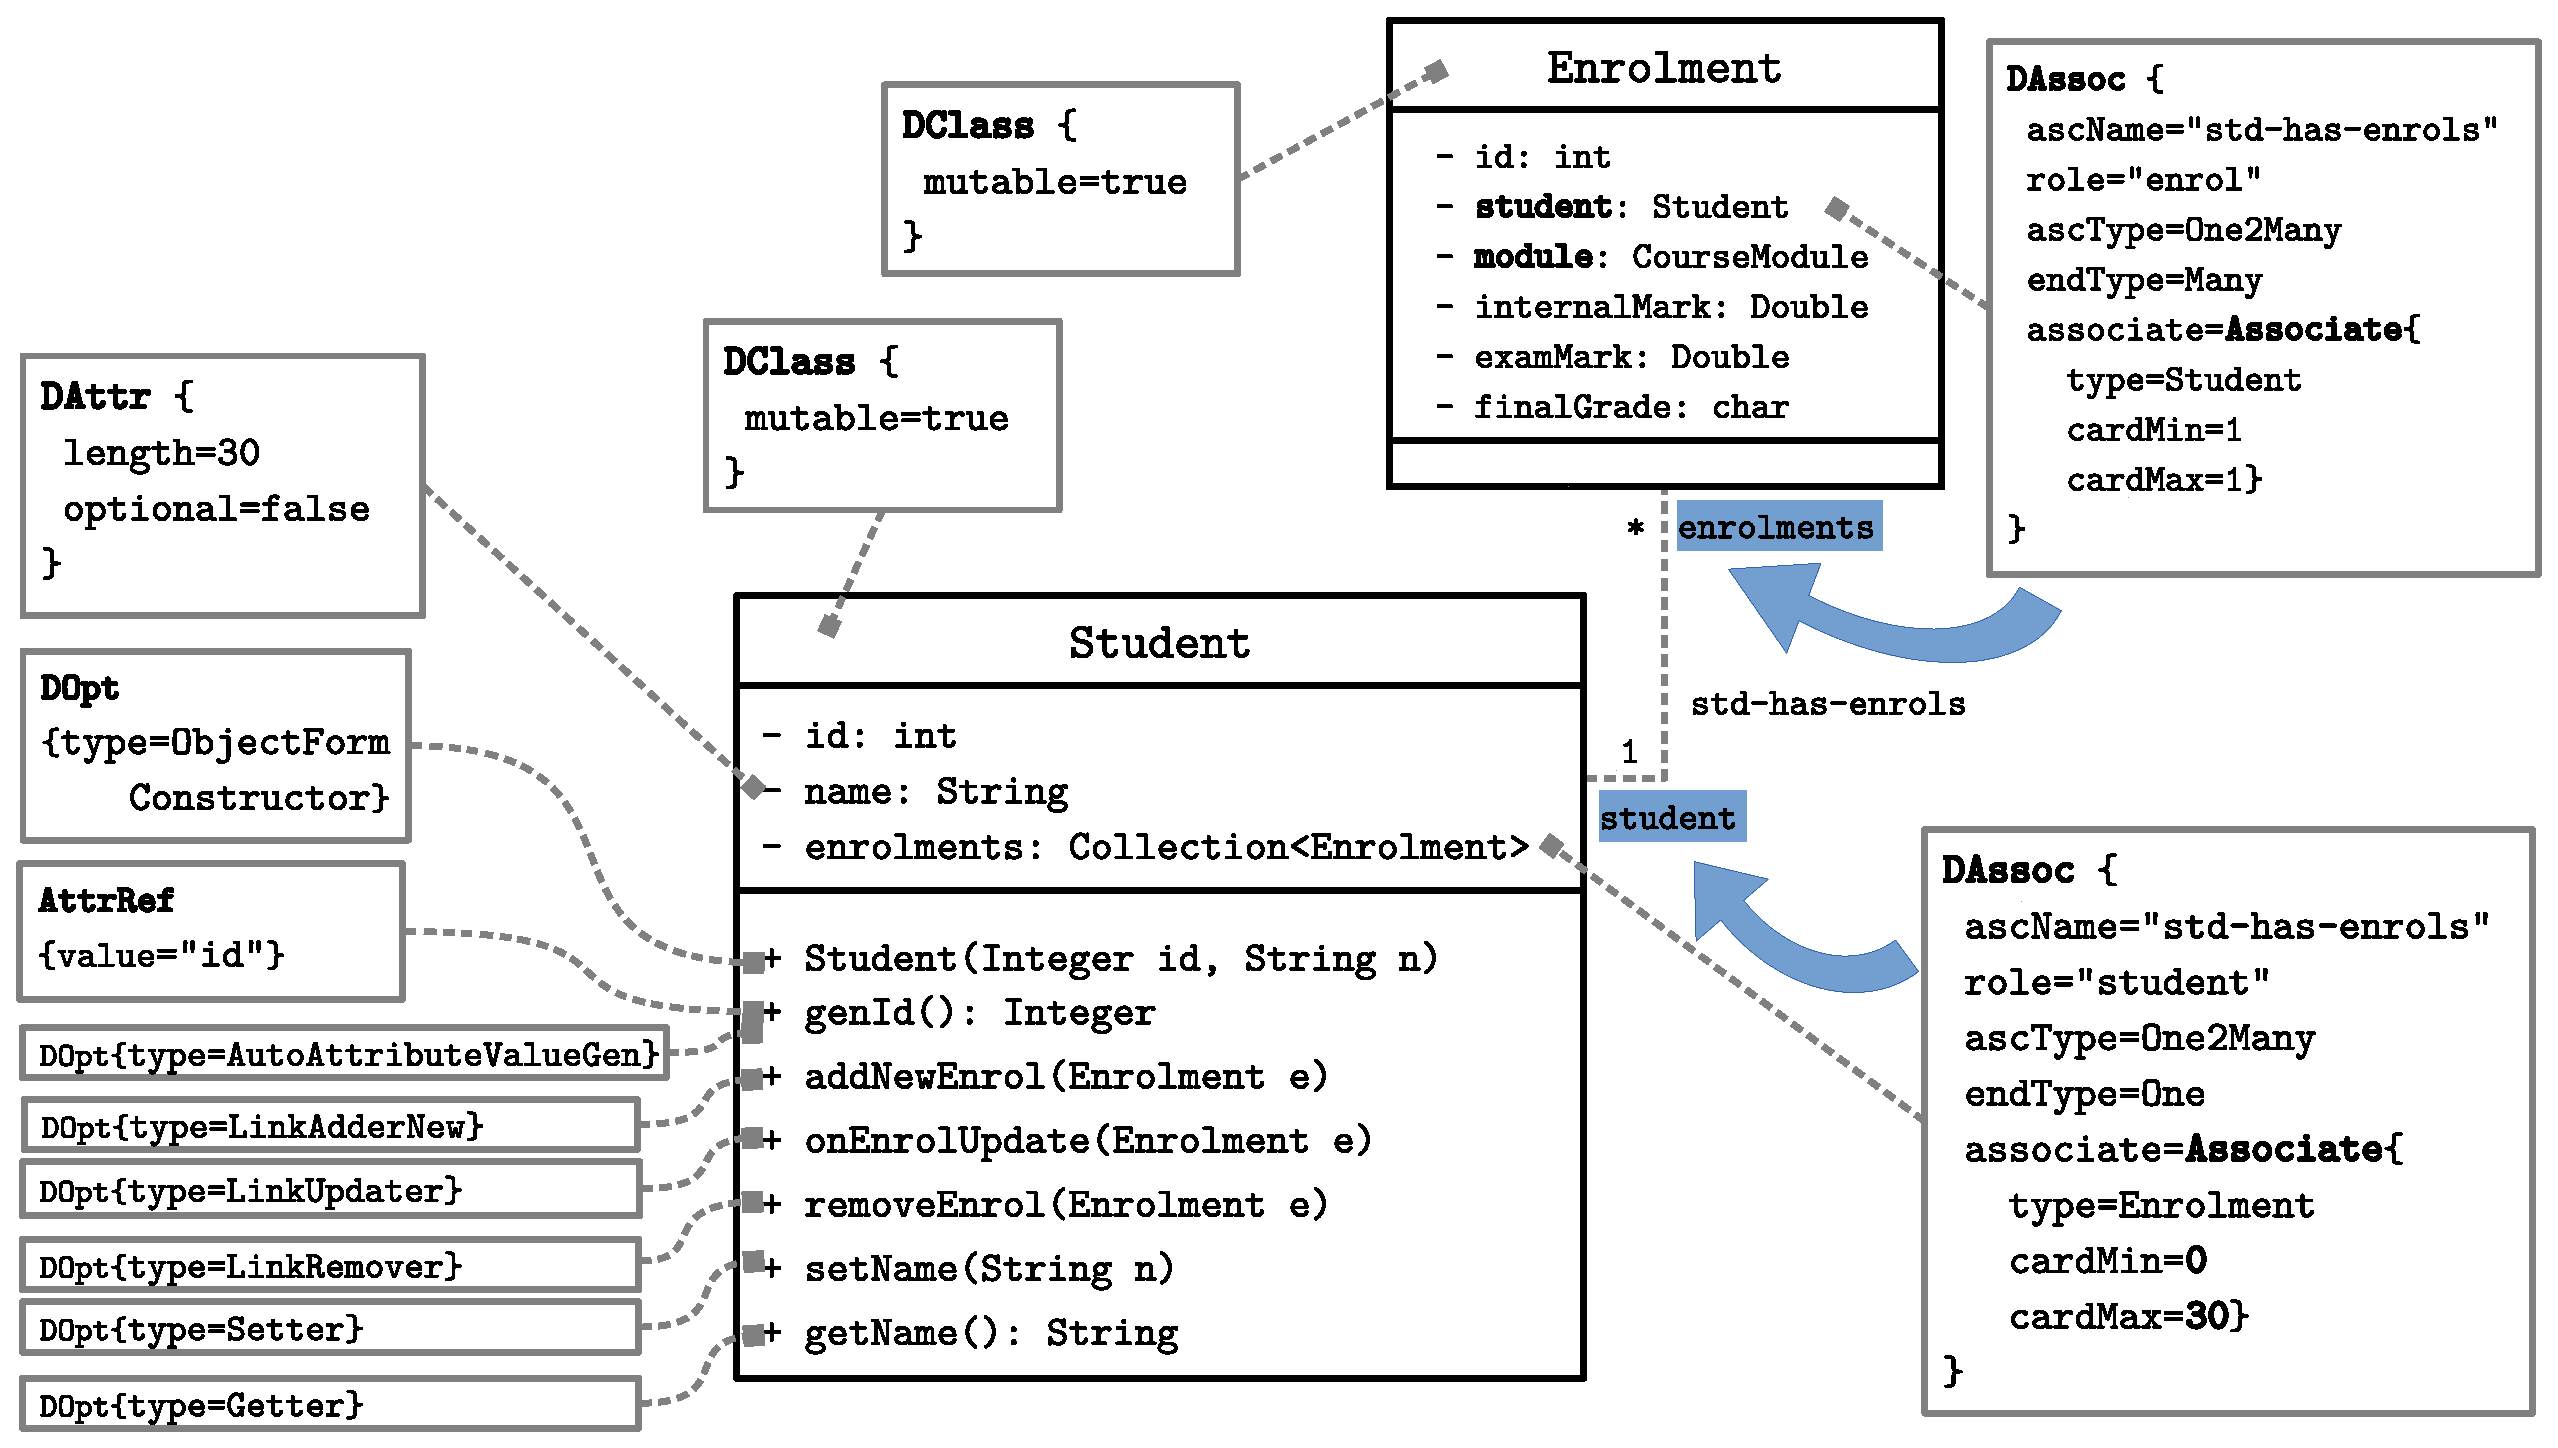
\includegraphics[scale=0.35]{dcsl-model-courseman}
	\caption{A partial \courseman domain model expressed in \dcsl~(adapted from~\cite{le_domain_2018}).}
	\label{fig:dcsl_courseman}
\end{figure}

For example, Fig.~\ref{fig:dcsl_courseman} shows a partial \courseman's domain model expressed in \dcsl. This model involves two domain classes: \clazz{Student} and \clazz{Enrolment}. Class \clazz{Enrolment} realises the many-many association between \clazz{Student} and \clazz{Course} (encapsulated by \clazz{CourseModule} as explained in SubSect~\ref{sect:bg-arch}). Both \clazz{Student} and \clazz{Enrolment} are assigned with a \clazz{DClass} element, which state that they are mutable domain classes. In particular, class \clazz{Student} has three domain fields: \attribn{id}, \attribn{name}, and \attribn{enrolments}. Domain field \attrib{Student}{name} is illustrated with an \clazz{DAttr} element which states that it is an optional domain field, whose maximum length is 30 (characters). An optional domain field means that the value of this field needs not be initialised when an object is created. Domain field \attrib{Student}{enrolments} is an associative field, which is assigned with a \clazz{DAssoc} element. This element specifies the \clazz{Student}'s end of the association with \clazz{Enrolment}. The opposite end of this association is specified by another \clazz{DAssoc} element that is assigned to the associative field \attrib{Enrolment}{student}. The two thick arrows in the figure map the two \clazz{DAssoc} elements to the two association ends. 
%
The seven methods of class \clazz{Student} listed in the figure are domain methods. Each method is assigned with a \clazz{DOpt} element, which specifies the behavior type. For instance, method \clazz{genId}, whose behavior type is \code{AutoAttributeValueGen}, is additionally assigned with an \clazz{AttrRef} element, which references the name of domain field \attrib{Student}{id}. This means that \clazz{genId} is the method that automatically generates values for \attrib{Student}{id}.

%%%%%%%%%%%%%%%%%%%%%%%%%%%%%%%%%%%%%%%%%%%%%%
\subsection{The Module-Based Software Architecture MOSA}
\label{sect:bg-arch} %
%%%%%%%%%%%%%%%%%%%%%%%%%%%%%%%%%%%%%%%%%%%%%%

To construct DDD software from the domain model requires an architectural model that conforms to the generic layered architecture~\cite{evans_domain-driven_2004, vernon_implementing_2013}. A key requirement of such model is that they position the domain model at the core layer, isolating it from the user interface and other layers. Evans~\cite{evans_domain-driven_2004} suggests that the MVC architecture model~\cite{krasner_description_1988} is one such model. The existing DDD frameworks~\cite{dan_haywood_apache_2013,paniza_learn_2011} supports this suggestion by employing some form of MVC architecture in their designs. We observe from all of these works that the user interface plays an important role in presenting a view of the domain model to the stakeholders in such a way that help them to effectively build the domain model. We thus argue that the MVC architecture must be backbone of any DDD tool that conforms to the DDD's layered architecture. 

Our previous works~\cite{le_tree-based_2015, le_generative_2018} propose a variant of the MVC architecture for DDD software, called \abbrv{module-based software architecture}{MOSA}. A key feature of this architecture is that it supports the automatic generations of software modules from the domain model and of the software from these modules.
%
A \textbf{MOSA model} consists in a set of MVC-based module classes. 
A \textbf{module class} is an MVC-based structured class~\cite{omg_unified_2015} that represents modules. This class is composed of three components: a domain class (the model), a view class (the view) and a controller class (the controller). The module class becomes the \textit{owner} of the model, view and controller. The view and controller are parameterised classes that are created by binding the template parameters of two library template classes, named \clazz{View} and \clazz{Controller} (\resp), to the domain class.
%
We present in~\cite{le_generative_2018} a technique for semi-automatically generating a module class from the domain class that it owns. Further, the view is designed to reflect the model structure. A set of module classes are used as input for the \jdomainapp~software framework~\cite{le_jdomainapp_2017} to automatically generate a software. In this paper, we will assume that a module class is defined for every domain class.

\begin{figure}[ht]
	\centering
	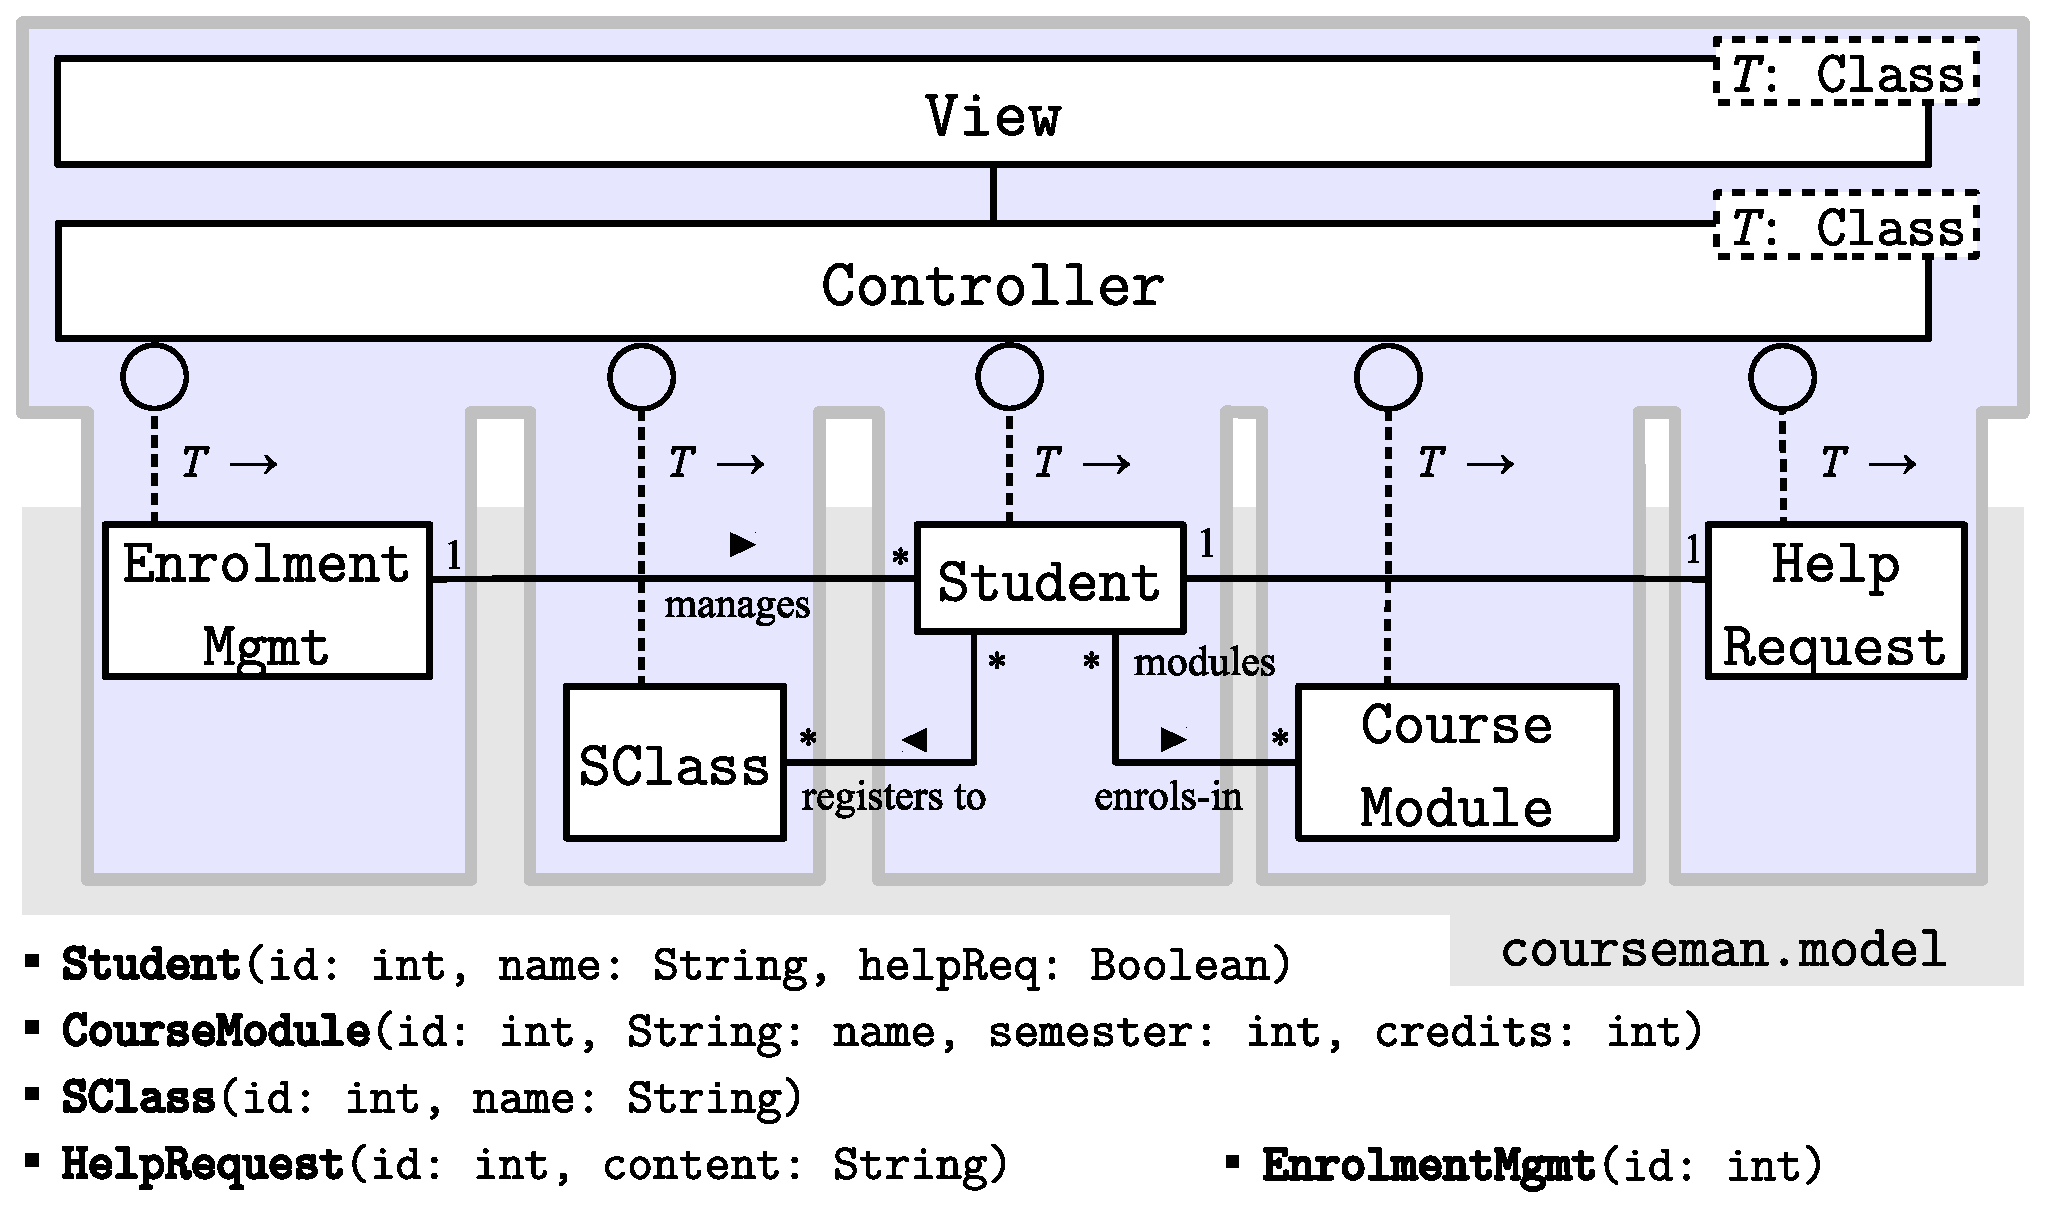
\includegraphics[scale=0.33]{sw-arch/arch-model-courseman}
	\caption{The MOSA model of \courseman.} %
	\label{fig:arch-model-courseman}
\end{figure}

%
To illustrate, the top-half of the MOSA model in Figure~\ref{fig:arch-model-courseman} shows five module classes of \courseman. The parameter bindings are depicted by dashed lines, whose \clazz{Controller}'s and \clazz{View}'s ends are drawn with the symbol `$\bigcirc$'. 
%
%To ease discussion, we name the module classes after their domain classes using the prefix \strq{Module}.
For example, the module class \clazz{ModuleStudent} is composed of three component classes: the domain class is \clazz{Student}, the view is \clazztemplate{View}{\clazz{Student}} and the controller is \clazztemplate{Controller}{\clazz{Student}}.

We argue that MOSA captures the essence of object-oriented software design in a modular, MVC-based design structure. According to Booch~\cite{booch_object-oriented_1986}, an object-oriented software consists in objects and their interactions that are realized though behavior invocation. Given that the domain model is expressed in \dcsl, the MOSA model that has this model at its core helps produce software that possesses the essential behaviors. First, objects are instances of the domain classes in the domain model, which are represented in \dcsl~with the essential structural features. Second, interaction among the objects of a group of domain classes is performed through an event-based message passing mechanism that is managed by the owner modules of these domain classes. This mechanism, which is described in detail in~\cite{le_jdomainapp_2017}, maps events to the essential behaviors that are supported in \dcsl. The events can be triggered by the user interaction on the view of a concerned module. 

However, in~\cite{le_domain_2018} we scoped our use of MOSA at the boundary of the domain model and assumed that this model is connected to the rest of MOSA model via activity graph. To express this graph in the context of MOSA requires exposing the component interface of the software modules and connecting this interface to the graph. We call this interface the module interface and discuss its design in Section~\ref{sect:actSemantics}. 
%We propose a language for expressing activity graphs in Section~\ref{sect:agl}.

%%%%%%%%%%%%%%%%%%%%%%%%%%%%%%%%%%%%%%%%%%%%%%
\subsection{Motivating Questions}
%%%%%%%%%%%%%%%%%%%%%%%%%%%%%%%%%%%%%%%%%%%%%%

As illustrated by the motivating example, a unified domain model could be defined as a loose combination of (1)~a class diagram for a domain model, (2)~an activity diagram for domain behaviors, and (3)~OCL constraints attached to these specifications. This puts forward a need to incorporate domain behaviors into the domain model specified by the DCSL framework~\cite{le_domain_2018} for a unified model with the three features, as explained in Section~\ref{sect:bg-dcsl}, feasibility, productivity, and understandability. Note that the DCSL framework has been defined as an initial effort for the three key features by extending the class metamodel with new meta-concepts to express OCL-like constraints.
%in the form of annotations in the host language.
Specifically, to realize this approach, we need to tackle the following challenges:

\begin{itemize}
    \item How can we extend the DCSL framework with new constructs to represent domain behaviors that could be captured by UML activity diagrams?
    \item How can we define a mechanism to incorporate such domain behaviors into a DCSL-specified domain model? This requires us to define an integrated semantics of structural and behavioral aspects of a domain model.
\end{itemize}


